% CVPR 2022 Paper Template
% based on the CVPR template provided by Ming-Ming Cheng (https://github.com/MCG-NKU/CVPR_Template)
% modified and extended by Stefan Roth (stefan.roth@NOSPAMtu-darmstadt.de)

\documentclass[10pt,twocolumn,letterpaper]{article}

%%%%%%%%% PAPER TYPE  - PLEASE UPDATE FOR FINAL VERSION
%\usepackage[review]{cvpr}      % To produce the REVIEW version
%\usepackage{cvpr}              % To produce the CAMERA-READY version
\usepackage[pagenumbers]{cvpr} % To force page numbers, e.g. for an arXiv version

% Include other packages here, before hyperref.
\usepackage{graphicx}
\usepackage{amsmath}
\usepackage{amssymb}
\usepackage{booktabs}


% It is strongly recommended to use hyperref, especially for the review version.
% hyperref with option pagebackref eases the reviewers' job.
% Please disable hyperref *only* if you encounter grave issues, e.g. with the
% file validation for the camera-ready version.
%
% If you comment hyperref and then uncomment it, you should delete
% ReviewTempalte.aux before re-running LaTeX.
% (Or just hit 'q' on the first LaTeX run, let it finish, and you
%  should be clear).
\usepackage[pagebackref,breaklinks,colorlinks]{hyperref}


% Support for easy cross-referencing
\usepackage[capitalize]{cleveref}
\crefname{section}{Sec.}{Secs.}
\Crefname{section}{Section}{Sections}
\Crefname{table}{Table}{Tables}
\crefname{table}{Tab.}{Tabs.}


%%%%%%%%% PAPER ID  - PLEASE UPDATE
\def\cvprPaperID{*****} % *** Enter the CVPR Paper ID here
\def\confName{CVPR}
\def\confYear{2023}


\begin{document}

%%%%%%%%% TITLE - PLEASE UPDATE
\title{Visual Geo-Localization:
mapping images to GPS}

\author{Cambria Paolo - s301164\\
Politecnico di Torino\\
{\tt\small paolocambria@studenti.polito.it}
\and
Ciciriello Giuseppe - s301953\\
Politecnico di Torino\\
{\tt\small giuseppe.ciciriello@studenti.polito.it}
\and
Testa Mario - s292630\\
Politecnico di Torino\\
{\tt\small mario.testa@studenti.polito.it}
}

\maketitle

%%%%%%%%% ABSTRACT
\begin{abstract}
Visual Geo-localization (VG) is the task of estimating the position where a given photo was taken by comparing it with a large database of images of known locations.
In this work, we investigate the results of CosPlace~\cite{Berton_CVPR_2022_CosPlace} in the task of Visual Geo-Localization. Their method casts the training as a classification problem and achieves state-of-the-art performances on a wide range of datasets and domain changes. We conducted a thorough ablation study of the loss function by comparing it with SphereFace~\cite{sphereface} and ArcFace~\cite{arcface} loss functions. Moreover, we carried out experiments on Domain Adaptation and Model Ensemble showing how a hybrid generative-discriminative approach helps robustness across domains, with special focus to the night one.
Finally, we assessed the behavior of our best model in a qualitative way, showing the correct reasoning in the image retrieval task.
Dataset, code and trained models are available for research purposes at: \newline
\url{https://github.com/Spidersaw/AML23-CosPlace/}
\end{abstract}


%%%%%%%%% BODY TEXT
\section{Introduction}\label{sec:introduction}
Visual geo-localization (VG) is one of the most promising approaches in the field of computer vision and image localization,
due to his importance in applications such as autonomous driving~\cite{6906961} or even augmented reality~\cite{middelberg}.
VG usually consists of a place recognition task: given a query image of a place, its geographical location has to be roughly recognized and retrieved
by finding the closest database geo-tagged images usually with a tolerance of few meters. 
This task is extremely challenging due to the intrinsic dynamism of public places and different problems must be taken in account:
there are a lot of moving objects which determine occlusion, environmental changes, different illuminations during daylight and night time, season changing.
Furthermore, most of the recent learning based VG methods focus on recognizing the location of images in a relatively small sized geographical area (\eg a neighborhood), 
which is not enough for real-world applications which are posed to operate at much larger scale (\eg whole cities).
\newline
\textbf{Non-representative datasets.}
To achieve a VG task on a wider geographical area, a large representative dataset is required and, as underlined by~\cite{Berton_CVPR_2022_CosPlace}, the majority of 
current datasets are either too small in the geographical coverage~\cite{netvlad,lidards,kittids}, or too sparse \cite{oxfds, mapillary}. Moreover, those datasets split the collected images into 
disjoint sets for training and inference and this not suits a realistic use case, since the search query might be often an already seen place.
For this reason it is recommendable to use the whole dataset to train the model, given also the cost of collecting the images for a consistent dataset.
\newline
\textbf{Training scalability.}
Having access to a massive amount of data raises the question of how to use it effectively for training. Many of the recent SOTA (state-of-the-art) methods take advantage
of contrastive learning ~\cite{netvlad, adageo}, which can often depend on contrasting positive to negative examples across the training dataset, a costly operation in terms of computation. CosPlace~\cite{Berton_CVPR_2022_CosPlace}, instead, addresses this limitation by using:
\begin{itemize}
    \item a new large-scale and dense dataset, called San Francisco eXtra Large (SF-XL), which includes multi-domain queries.
    \item a highly scalable training method, properly designed to work on large dataset, based on a classification task to produce a model that will later be used to extract descriptors for the retrieval
\end{itemize}
successfully reaching SOTA results with compact descriptors.
\newline
\textbf{Contributions.}
In this paper we want to investigate how the work of~\cite{Berton_CVPR_2022_CosPlace} can be improved for place recognition tasks, but using a smaller version of SF-XL dataset (called SF-XS) for the training, due to our limited resources.
In particular we focus on:
\begin{itemize}
    \item generally improve the recalls on SF-XS and Tokyo-XS (a smaller version of Tokyo 24/7~\cite{tokyo247}), even with the help of ensembles to concatenate the descriptors of different models.
    \item improve robustness to domain shift by borrowing techniques from the field of domain adaptation~\cite{adageo}, and testing the results on a dataset which only contains night images, called Tokyo-Night (a filtered version of Tokyo-XS) and deeply understanding the applied domain adaptation techniques.
    \item assess how CosPlace behaves when data quality is scarce (\eg occlusion and blurry photos). 
\end{itemize} 

Through some experiments, we demonstrate that our solution exceeds the baseline provided by CosPlace on three different datasets and that the core ideas of the architecture (data augmentation, both domain-driven and non, and subsequent domain adaptation) provide modest increments to the performance.

%-------------------------------------------------------------------------
\section{Related Works}\label{sec:relatedworks}
\textbf{Visual geo-localization as image retrieval.} Visual geolocalization on large scale is commonly considered as an image retrieval task, in which the correctness is determined by an established
tolerance (usually 25 meters) from the query's ground truth position~\cite{netvlad, adageo}.    
One of the most representative study in this field is NetVLAD~\cite{netvlad}, which introduces a VLAD layer, which has parameters learnable with back-propagation, that pools descriptors extracted from a CNN backbone into a fixed image representation.
\newline

\textbf{Visual geo-localization as classification.}
An alternative approach to visual geo-localization is to consider it a classification problem, as done in~\cite{Berton_CVPR_2022_CosPlace}. Most of methods of this kind, divide the geographical area of interest in cells and group the database of images in classes according to their cell, which has a big limitation: nearly identical images may be assigned to different classes due to quantization errors.
CosPlace, instead, proposes to train the model only using groups of non adjacent classes and iterates over them while using CosFace~\cite{cosface} as a scalable loss.
\newline

\textbf{Deep Face Recognition.}
In deep face recognition (FR) problem under open-set protocol, ideal face features are expected to have smaller maximal intra-class distance than minimal inter-class distance under a suitably chosen metric space. Different methods~\cite{sphereface, cosface, arcface} have shown how learning angularly discriminative features on a hypersphere manifold with an adjustable margin helps to improve accuracy on both verification and identification tasks. The most representative studies in this field are SphereFace~\cite{sphereface} which uses a multiplicative angular margin inside the loss function, CosFace~\cite{cosface} which applies an additive cosine margin directly to the target logits and ArcFace~\cite{arcface} which applies an angular margin that exactly corresponds to the geodesic distance. [TODO Non mi piace tanto com'è scritta la descrizione di sphere, cos e arc...]
\newline

\textbf{Unsupervised domain adaptation.}
Unsupervised domain adaptation attempts to reduce the shift between the source and target distribution of the data by relying only on labeled source data and unlabeled target data. For example, the source domain can consist of synthetic images and their corresponding pixel-level labels (\eg for semantic segmentation), and the target can be real images with no ground-truth annotations. One approach for unsupervised domain adaptation is to learn domain-invariant features from the data, it was introduced by~\cite{grl} and is based on a domain discriminator network with a gradient reversal layer (GRL) that forces feature extractor to produce domain-invariant representations. This has been used by AdaGeo-Lite~\cite{adageo} architecture, which combines a domain-driven data augmentation module that uses a non-learned style transfer method (called FDA~\cite{fda}) producing a pseudo-target labeled dataset, with a network that produces domain-invariant image descriptors by setting up a min-max game where the discriminator tries to minimize the domain classification loss given three datasets (source, pseudo-target and a few samples from the target domain), while the feature extractor acts as an adversary to the discriminator.

%----------------------------------------------------------------


%-------------------------------------------------------------------------
\section{Method}\label{sec:experiments}
In this section, we present different approaches we have used to try improving CosPlace results. We started from its original implementation and decided to add custom augmentation to help boost its ability to learn embeddings even on sub-optimal picture quality. Then, we moved our focus to domain shift, given that test-images are likely to come from different domains than the source and that the domain shift in the dataset of interest Tokyo-Night is caused by illumination (day/night), we tried adapting the method used by~\cite{adageo} combined to CosPlace in order to create a modular architecture composed of two parts:
\begin{itemize}
    \item A non-learned domain-driven data augmentation module that transfer the style of the target domain (night) to the source images.
    \item A network that produces the image descriptors, composed of a CNN, an aggregation layer and domain adaptation module.
\end{itemize}
At the end, we tried averaging the weights of models trained in the previous steps using Model Soups' approach~\cite{modelsoup} to improve recalls.

\begin{figure*}
  \centering
  \begin{subfigure}{0.58\linewidth}
    \fbox{
   
    \begin{tabular}{ccc}
      \includegraphics[width=25mm]{assets/gridof6/example1.jpg} &   \includegraphics[width=25mm]{assets/gridof6/example2.jpg} &
      \includegraphics[width=25mm]{assets/gridof6/example3.jpg}\\
     \includegraphics[width=25mm]{assets/gridof6/example4.jpg} &   \includegraphics[width=25mm]{assets/gridof6/example5.jpg} &
      \includegraphics[width=25mm]{assets/gridof6/example6.jpg}\\
    \end{tabular}

    }
    \caption{Example of images from San Francisco XS dataset: they cover different time \\of the day, weather conditions, viewpoint and occlusions.}
    \label{fig:short-a}
  \end{subfigure}
  \hfill
  \begin{subfigure}{0.38\linewidth}
    \fbox{\rule{0pt}{1.5in} 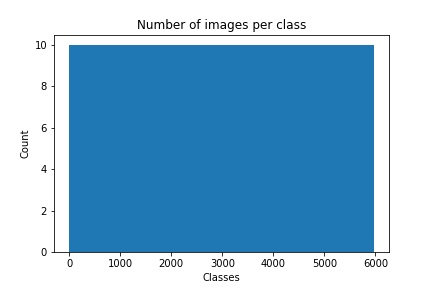
\includegraphics[width=0.9\linewidth]{assets/no_images_per_class.jpeg}}
    \caption{Numbers of images per class in San Francisco XS dataset.}
    \label{fig:sfxs_density}
  \end{subfigure}
  \caption{Example of a short caption, which should be centered.}
  \label{fig:short}
\end{figure*}

\subsection{Datasets}
For our work, we have been provided with two datasets to experiment with: San Francisco eXtra Small (\textbf{SF-XS}) and Tokyo eXtra Small (\textbf{Tokyo-XS}). These datasets are respectively subsets of SF-XL~\cite{Berton_CVPR_2022_CosPlace} and Tokyo 24/7~\cite{tokyo247} purposely reduced for our convenience due to limitations in compute availability. SF-XS contains 59704 images for the train (both queries and database), 16008 for the evaluation (8015 as database, 7993 as queries) and 28191 for the test (27191 as database, 1000 as queries).
Tokyo-XS only contains 13086 images for the test (12771 as database, 305 as queries).
All these datasets are provided with labels that can be derived from the images' names as \textit{\{east, north, heading\}} and specifically for the training dataset, there are 5965 different classes, each one of them containing 10 images, as shown in \cref{fig:sfxs_density}.
Finally, to understand if the changes applied to our model help in geolocalizing night images, we created a new dataset called \textbf{Tokyo-Night}: it is a subset of Tokyo-XS of which only the night images from queries are retained (1 out of 3, so 105 query images in total).


\subsection{CosPlace}
Our work starts from CosPlace, an innovative approach in the field of visual geo-localization~\cite{Berton_CVPR_2022_CosPlace}. CosPlace casts the network training as an image classification problem: it partitions the geographical area of interest in oriented cells, representing different classes, using UTM coordinates $\{east,north\}$\footnote{UTM coordinates are defined by a system used to identify locations on earth in meters, where 1 UTM unit corresponds to 1 meter. They can be extracted from GPS coordinates (i.e., latitude and longitude) and allow approximating a restricted area of the earth’s surface on a flat surface.} and orientation/heading $\{heading\}$. The extent of each class in terms of position and heading is defined by two parameters $M$ and $\alpha$, respectively. Then, it iteratively considers subsets of these cells (called groups $G_{uvw}$) to train the network.
These groups are generated by fixing the minimum spatial separation that two classes of the same group should have, either in terms of translation or orientation. For this reason, they introduced two parameters: $N$ controls the minimum number of cells between two classes of the same group, and $L$ is the equivalent for the orientation.
Therefore, we have trained sequentially over the groups as:
\begin{equation}
  \mathcal{L}_{cosPlace} = \mathcal{L}_{lmcl}(G_{uvw})
  \label{eq:cosplace_full}
\end{equation}
where $\mathcal{L}_{lmcl}$ is the Large Margin Cosine Loss as defined in~\cite{cosface}, and $u \in \{0,...,N\}, v \in \{0,...,N\}, w \in \{0,...,L\}$ represent the different values of $\{east, north, heading\}$. In our case, due to limitations in compute availability, we could only train each epoch on the same group $G$, so:
\begin{equation}
  \mathcal{L}_{cosPlace} = \mathcal{L}_{lmcl}(G)
  \label{eq:cosplace_our}
\end{equation}
At validation and test time, we used the model generated not to classify the query, but rather to extract image descriptors as in~\cite{cosface} for a classic retrieval over the database. This allows for the model to be used also on other datasets from unseen geographical areas, like Tokyo-XS and the smaller Tokyo-Night.

\begin{figure*}
  \centering
  \begin{subfigure}{1.0\linewidth}
    \centering
    \fbox{ \includegraphics[width=\dimexpr\textwidth-2\fboxrule-2\fboxsep]{assets/architecture.png}}
  
  \end{subfigure}
     \caption{The proposed architecture. First, a domain-driven data augmentation method is used to generate a labeled pseudo-target dataset from the source dataset and just 5 unlabeled target images. Then, the source dataset, pseudo-target dataset, and the 5 unlabeled target images are used to train the network that extracts the image descriptors. This network leverages an aggregation module and a domain adaptation module to provide robustness to shifting.}
    \label{fig:our_architecture}
  \hfill
\end{figure*}


\subsection{Custom Augmentations}
To assess the robustness of CosPlace~\cite{Berton_CVPR_2022_CosPlace}, its capability to learn a good embedding space even on sub-optimal picture quality and try to find augmentations to achieve better generalization,
we conducted a study on the augmentation pipeline already present in the original implementation. Following SFRS \cite{sfrs} during the training step (Color Jitter, RandomResizedCrop, Normalize) that we named \textbf{base}, we added 4 new augmentations on the images after the default Color Jittering, with a 25\%  chance of being applied and a fixed seed for reproducibility purposes. Those augmentations consisted of:
\begin{itemize}
  \item \textbf{Gaussian Blur}\newline
Blurring images can show the robustness of CosPlace on realistic use case in which the provided images are not always clear.
  \item \textbf{Grayscale}\newline
  In the context of place recognition Grayscale has already been successfully employed in \cite{grayscalecnn} to reduce the effect of illumination variation, which suits also our case.
  \item \textbf{Horizontal Flip}\newline
The datasets in use contain informations on orientation and heading of the images, applying an horizontal flip should prove consistency on the query images. 
  \item \textbf{Erasing}\newline
Randomly erasing an amount of pixels in the picture, can simulate the realistic case of occlusion and usually improves the CNN-based recognition models as \cite{reda}.
\end{itemize}


\begin{figure}[b]
    \centering
    \fbox{ 
    \begin{tabular}{cc}
  \includegraphics[width=35mm]{assets/source-example.jpg} &   \includegraphics[width=35mm]{assets/pseudo-example.jpg} \\
  \end{tabular}
  }
    \caption{On the left the source image, on the right the pseudo-target image generated with FDA + saturation and temperature convertion.}
    \label{fig:fda_show}
\end{figure}

\subsection{FDA and GRL}
\textbf{Domain-Drive Data Augmentation.}
The purpose of the domain-driven data augmentation (DDDA) module is to find a mapping $D_s \mapsto D_{pt}$ from the source domain to a pseudo-target domain that better approximates the target domain, i.e., $D_{pt} \approx D_t$. This mapping can then be applied to the source dataset $X_s$ to generate a new labeled dataset with pseudo-target images $X_{pt}$, it is a data augmentation technique and is performed only once, offline. Inspired by~\cite{fda, adageo}, we used a DDDA method based on Fourier Domain Adaptation (\textbf{FDA})~\cite{fda} to generate a pseudo-target dataset $X_{pt}$ given two randomly sampled images $x^s$ and $x^t$ from source and target. First, the low frequency part of the amplitude of $x^s$ is replaced by that of $x^t$, then the modified spectral representation of the source is mapped back to an image whose content is the same as $x^s$ but will resemble the appearance of a sample from the target distribution.
Since the pseudo-target images generated didn't look as "night" as thought, for all the processed images, we reduced their saturation to 70\% and converted their temperature towards blue, to give them a colder appearance, as shown in~\cref{fig:fda_show}
Afterward, we use both $X_s$ and $X_{pt}$ to train the descriptor extraction network, leading to a more robust model.
\newline

\textbf{Domain Adaptation Module.}
In order for the retrieval to work well across domains it is important that the embeddings produced by the descriptor extraction network are domain agnostic, i.e., they do not encode domain-specific information. We achieve this by using a domain discriminator which receives embeddings from the three domains $D_s$, $D_pt$, and $D_t$. The discriminator is composed of two fully connected layers, and its goal is to classify the domain to which the embeddings belong. Just before the discriminator, there is a gradient reversal layer (\textbf{GRL})~\cite{grl} that in the forward pass acts as an identity transform, while in the backward pass multiplies the gradient by -$\lambda$, where $\lambda > 0$. The use of this layer effectively sets up a min-max game, where the discriminator tries to minimize the domain classification loss, that is a cross-entropy loss $L_{CE}$, while the feature extractor learns to produce domain-invariant embeddings, acting as an adversary to the discriminator.
\newline

\textbf{Architecture details.}
The idea is that for each input $x$, we predict its class $y \in Y$ and its domain label $d \in \{0, 1\}$, depending if it is an image from day or night.
We assume that the input $x$ is the output of the frozen layers of our CNN backbone, which we call feature vector $f$.
Then, we fine-tune the last layers of the CNN, the upper branch aggregator in \cref{fig:our_architecture} pools $f$ (if it comes from the labeled source) with GeM Pooling to finish the image descriptor extraction, and we denote the parameters of this section with $\theta_f$. Then the descriptor is mapped to its class label probabilities $y$ by CosFace, with parameters $\theta_y$. Finally, the same feature vector $f$ is mapped to the domain label $d$ by the lower branch in \cref{fig:our_architecture} (\textit{domain classifier}), with $\theta_d$ as parameters.
During the learning stage, we aim to minimize the label
prediction loss on the labeled part (i.e. the source part)
of the training set, and the parameters of both the feature
extractor $\theta_f$ and the label predictor $\theta_y$ are thus optimized in order to minimize the cross-entropy loss for the source domain samples $L_y$. At the same time, to make the features $f$ domain-invariant we seek $\theta_f$ that maximize the loss of the domain classifier $L_d$, while simultaneously seeking $\theta_d$ that minimizes the latter. The trade-off between the two objectives is controlled by a parameter $\lambda$. The parameters update are similar to the ones of stochastic gradient descent (SGD) for a feed-forward deep model that
comprises feature extractor fed into the label predictor and
into the domain classifier, but the difference here is given from $\lambda$ so a direct implementation of SGD is not possible. This can, instead, be accomplished by a Gradient Reversal Layer (GRL)  which during the forward propagation acts as an identity transform and during the backpropagation takes the gradient from
the subsequent level, multiplies it by $-\lambda$ and passes it to
the preceding layer.
At the end of the training phase, the two losses ($L_y$, $L_d$) are combined as $L_y + \alpha \cdot L_d$ where $\alpha = 0.1$.

\subsection{Model Soup}
Training a learning model is usually done in two steps: first, the model is trained several times by varying the hyper parameters, and then the model with the best performance is chosen before being used. 
The publication ”Model soups: averaging weights of multiple fine-tuned models improves accuracy without increasing inference time”~\cite{modelsoup} proposes to average the weights of the different models to maximize the use of all the training [TODO training cosa??] without wasting learning time. This adds very little memory cost, learning time or inference time. The paper shows that a performance increase is visible on some models and even defines a new state of the art on image classification. The authors present two ways to combine two (or more) models to create a soup: greedy soup and uniform soup. In this project we tried to implement greedy version of the proposed solution and then we test the model on the datasets available.
[TODO] Insert here description of how Model Soup has been implemented.

\section{Experiments}
\textbf{Experiment with the Baseline.}
We started running some experiments to better understand how the training procedure worked. The backbone used was a ResNet-18 pre-trained on ImageNet with GeM pooling~\cite{finetuning} and due to limitations in compute availability (\eg Colab time and GPU limitations), we trained the baseline model for only 3 epochs to finally end up with the results in \cref{tab:baseline}:


\begin{table}[htp]
  \centering
  \begin{tabular}{@{}cccc@{}}
    \toprule
    & SF-XS(test) & Tokyo-XS & Tokyo-Night\\
    \midrule
    R@1/R@5 & \textbf{52.2/66.3} & \textbf{69.5/84.8} & \textbf{49.5/72.4} \\
    R@10 & 71.8 & 89.2 & 79.0\\
    R@20 & 76.3 & 92.7 & 84.4\\
    \bottomrule
  \end{tabular}
  \caption{Baseline results, values refer to recall@K, for K=\{1, 5, 10, 20\}}
  \label{tab:baseline}
\end{table}


\textbf{Ablation study when changing the angular loss function.}
Once we were familiar with the baseline, we started making a few modifications to the model, specifically to the loss function. Standard CosPlace uses the Large Cosine similarity loss~\cite{cosface}, so we've tried replacing it with two other alternative cosine based losses: SphereFace~\cite{sphereface} and ArcFace~\cite{arcface}.
We trained the modified version on SF-XS and the results in \cref{tab:lossablation} show how CosFace loss performs better than the competition on the biggest dataset (SF-XS), while on smaller ones (Tokyo-XS and Tokyo-Night) SphereFace and ArcFace actually get better recall values. This isn't what we expected at first, but further analysis suggest us that the implementations we've use for the last two losses might converge earlier than the original CosFace, so with a low number of epochs they perform better.
It would be interesting to have some trials with the full SF-XL dataset and a greater number of epochs to better understand the behavior in the long run.

\begin{table}[htp]
  \centering
  \begin{tabular}{@{}cccc@{}}
    \toprule
     & SF-XS(test) & Tokyo-XS & Tokyo-Night\\
    \midrule
    CosPlace with\\ CosFace & \textbf{52.2/66.3} & 69.5/84.8 & 49.5/72.4 \\
    CosPlace with\\ SphereFace & 49.7/64.2 & \textbf{70.2/84.8} & \textbf{59.0/75.2} \\
    CosPlace with\\ ArcFace & 49.7/61.1 & 69.5/81.6 & 56.2/64.8\\
    \bottomrule
  \end{tabular}
  \caption{Results of our ablation study when changing the angular loss function from CosFace to SphereFace and ArcFace, the values refer to Recall@1/Recall@5.}
  \label{tab:lossablation}
\end{table}

\textbf{Augmentation Pipeline.}
Due to the high computational requirements, we were only able to conduct this ablation efficiently on SF-XS dataset with a low amount of iterations per epochs fixed to 5000 and a batch size reduced to 16 instead of respectively 10000 and 32 as the default model. The results reporting recalls are presented in the table \ref{tab:augmentations-pp} below:

% ABLATION AUGMENTATIONS

\begin{table}[hbp] % Add the following just after the closing bracket on this line to specify a position for the table on the page: [h], [t], [b] or [p] - these mean: here, top, bottom and on a separate page, respectively
\centering % Centers the table on the page, comment out to left-justify
\begin{tabular}{l c c c c c} % The final bracket specifies the number of columns in the table along with left and right borders which are specified using vertical bars (|); each column can be left, right or center-justified using l, r or c. To specify a precise width, use p{width}, e.g. p{5cm}
\toprule % Top horizontal line
Augmentations & R@1 & R@5 & R@10 & R@20\\ % Column names row
\midrule % In-table horizontal line
Base & 43.9\%  & 61.7\% & 67.0\% & 71.2\%  \\ 
+\{blur\} & 44.2\%  & 60.4\% & 67.3\% & 70.8\%  \\ 
+\{grayscale\} & 45.6\%  & 60.9\% & 67.4\% & 70.7\%  \\ 
+\{flip\} & 43.8\%  & 62.0\% & 68.0\% & 71.9\%  \\  
+\{erasing\} & 44.0\%  & 59.8\% & 65.0\% & 70.2\%  \\  
+\{grayscale, erasing\} & 43.4\%  & 59.2\% & 65.2\% & 70.1\%  \\  
+\{blur, grayscale\} & 45.9\%  & 61.3\% & 68.6\% & 70.9\%  \\  
+\{blur, erasing\} & 43.8\%  & 60.2\% & 65.3\% & 70.4\%  \\  
+\{blur, grayscale,\\ flip, erasing\} & 43.6\%  & 59.1\% & 64.8\% & 70.4\%  \\  

\bottomrule % Bottom horizontal line
\end{tabular}
\smallskip 
\caption{Evaluation of the impact in terms of recall of different augmentation pipelines for CosPlace compared to Base (Color Jitter, RandomResizedCrop, Normalize)
} % Table caption, can be commented out if no caption is required
\label{tab:augmentations-pp} % A label for referencing this table elsewhere, references are used in text as \ref{label}
\end{table}

The couple of augmentation \textbf{blur, grayscale} seems the best choice for the augmentation pipeline, since not only the model manages to show robustness to that data augmentation pipeline, but also gets improvements.
Further investigations should be performed with different parameters (\eg number of iterations, batch size, augmentation intensity, etc.) to deeply understand their behavior, however it seems that applying grayscale to the model leads to better performances, since it might add invariance to the colors of the scenes changing through the day.
\newline

\textbf{Unsupervised Domain Adaptation with FDA and GRL.}
To evaluate the capability of our solution to generalize to unseen domains, specifically the night one, we compare the baseline, the unchanged architecture of the baseline trained with a dataset containing the source domain samples and target-domain samples generated with FDA, and the architecture with the domain discriminator module attached (FDA+GRL). In \cref{tab:fda+grl} we show the results for each method.

\begin{table}[htp]
  \centering
  \begin{tabular}{@{}cccc@{}}
    \toprule
    & SF-XS(test) & Tokyo-XS & Tokyo-Night\\
    \midrule
    Baseline & 52.2/66.3 & 69.5/84.8 & 49.5/72.4 \\
    FDA & 50.5/65.4 & 67.0/85.7 & 47.6/72.4 \\
    FDA+GRL & \textbf{53.7/66.5} & \textbf{70.5/84.8} & \textbf{53.3/73.3}\\
    FDA+GRL+g & 53.4/65.5 & 67.6/84.8 & 48.6/72.4\\
    \bottomrule
  \end{tabular}
  \caption{Baseline results compared with FDA only, FDA+GRL (with $\alpha=0.1$) and FDA+GRL+grayscale.}
  \label{tab:fda+grl}
\end{table}

From these results, we surpass the baseline in all the three datasets by using both FDA and GRL together, reaching a $\sim4\%$ improvement on Tokyo-night. This confirms that the newly generated model was able to produce "more" domain-invariant features than before, with the downside of increasing the training time. Better can be expected by trying out different values for $\alpha$ or maybe performing a better post processing on the pseudo-target images generated.
Finally, adding the best performing custom augmentation (grayscale with 25\% chance to be applied) didn't provide any improvement to the FDA+GRL model, showing that if real colors are available, they will outperform the generalization improvement of grayscale.
\newline

\textbf{Averaging model weights with Greedy soup algorithm.}
To maximize model accuracy of our solution we pick all the best models trained and then merge them in a single model capable to improve performances without increasing inference time.
The greedy soup is constructed by sequentially adding each model as a potential ingredient in the soup, and only keeping the model in the soup if performance on a held out validation set improves.
For this purpose we decided to sort the models in a decreasing order of their recall values got in the training step, in this way the soup have to be certainly better or equal than the best model analyzed. 
Unfortunately, due to Colab limitations (in terms of batch size and epochs number for the training step) we had a limited number of models to use and we didn't achieve any real improvement on our best model (FDA+GRL) after testing on all the datasets available. This can happen if every time the next model in the list is added, it gets discarded because it doesn't provide any performance increment. This could be one of the approaches to be further explored, in the future, with more advanced tools. 
\newline

\textbf{Qualitative Evaluation with Top K-NN.}
To assess the goodness of the results obtained applying FDA and GRL in particular on Tokyo-Night dataset, we look at the nearest neighbors in the feature space, to understand the trained model's reasoning on different proposed queries. 
Therefore, we built a top K - Nearest Neighbors visualization
for which given a query image, the K closest points in the learning embedding space are retrieved.
In order to retrieve the top K = 5 most similar images to a given one, we calculate the Euclidean distance between the target image's embedding and each image's embedding in the dataset, one by one.
For our experiment, we used and tested Tokyo-Night as database for the queries retrieval in fig. \cref{fig:tokyonighttopknn} in two different ways.
The model was trained with both FDA and GRL active, however:
\begin{itemize}
    \item in the set \textbf{A} we didn't apply FDA to the dataset used for the Top K-NN retrieval, just to be sure that our trained model worked as intended with the original set, both on day and night queries. The result was perfect for the first 3 neighbors.
    \item in the set \textbf{B} we applied FDA to the dataset used for the Top K-NN retrieval and used as queries the same image treated with FDA (on the left) and from the night domain (on the right).
    Once again the result was satisfactory and the FDA-treated image was perfectly recognized and integrated in both cases, proving the correct reasoning of our proposed model.
\end{itemize}

\begin{figure*}[t]
\centering
  \begin{subfigure}{1.0\linewidth}
    \centering
    \fbox{ \includegraphics[width=\dimexpr\textwidth-2\fboxrule-2\fboxsep]{assets/topknn.png}}
  \end{subfigure}
      \caption{Given a target image, top 5 matching images are shown. Preset A) corresponds to Tokyo-Night dataset without FDA applied.
Preset B) corresponds to Tokyo-Night dataset with FDA applied on the target image on the left.}
  \hfill
  \label{fig:tokyonighttopknn}
\end{figure*}

\section{Conclusions}
In this paper, we proposed different improvements to CosPlace.
In order to obtain better performances than the baseline on the night dataset, different from the training one for colors, brightness and city where the pictures were taken, we demonstrated that it is possible to improve domain shifting by applying FDA on the training dataset and using a Domain Adaptation module that forces the feature extractor to produce domain-invariant representations. We have also found that this solution improves the recalls of SF-XS and Tokyo-XS as well, and we assessed our results with a Top K-NN retrieval.
\newline
Furthermore, we confirmed our hypothesis of applying grayscale on images to improve illumination invariance.
\newline
Finally, we tried boosting recalls of our model with a Greedy Soup approach, but didn't get any enhancement or worsening.
\newline

We believe that this work can be still improved, possibly with the use of an attention layer before the aggregator, as done in~\cite{adageo} that, given this field and on top of our proposals, might show interesting results.


%%%%%%%%% REFERENCES
{\small
\clearpage
\bibliographystyle{IEEEtran}
\bibliography{egbib}
}

\end{document}
